
\section{Simulation}\label{sec:simulation}
% Simulation:
%%  Mean control results   (image and plot(s) )
%%  Variance Control      (image and plot(s) )
%%  Hybrid control   (image and plot(s) )

\subsection{Controlling the mean position}

For controlling mean position, we use a PID controller. Our control input is the force we make, goal positions are the desired positions, and we have our mean position and mean velocity. So we have:
\begin{align}
control\_input_x &= K_{g}*(goal_x - \bar{x}) + K_{d}*(0-\bar{v}_x) \nonumber\\
control\_input_y &= K_{g}*(goal_y - \bar{y}) + K_{d}*(0-\bar{v}_y) 
\end{align}
where Kgain is the gain value, and Kderivative is the derivative value. In order to find these gain values, we tried different values to find the best between them as shown in figure ???.
In this experiment 100 robots were used and the maximum speed would be 3 cell per second. And with these parameters, we showed that the best values for Kgain is 4, and the best value for Kderivative is 1.


%give PID control law, explain experiment (number of robots, maximum speed, ).

%contrast controllers -- as is typical with PID control laws, we can tune the response to meet desired specifications.


%image showing varying P control  %I want  1.5 cycles, nicely cropped,  all starting at same time

%image showing varying D control

%image showing varying the number of robots n % is this needed?

%\subfloat[][Vary Visual Feedback]{\label{fig:VaryVis}
%\begin{overpic}[width =\figwid]{VaryVisFS.pdf}\end{overpic}}


%\begin{figure}
%        \centering
%        \begin{subfigure}[b]{0.3\textwidth}
%                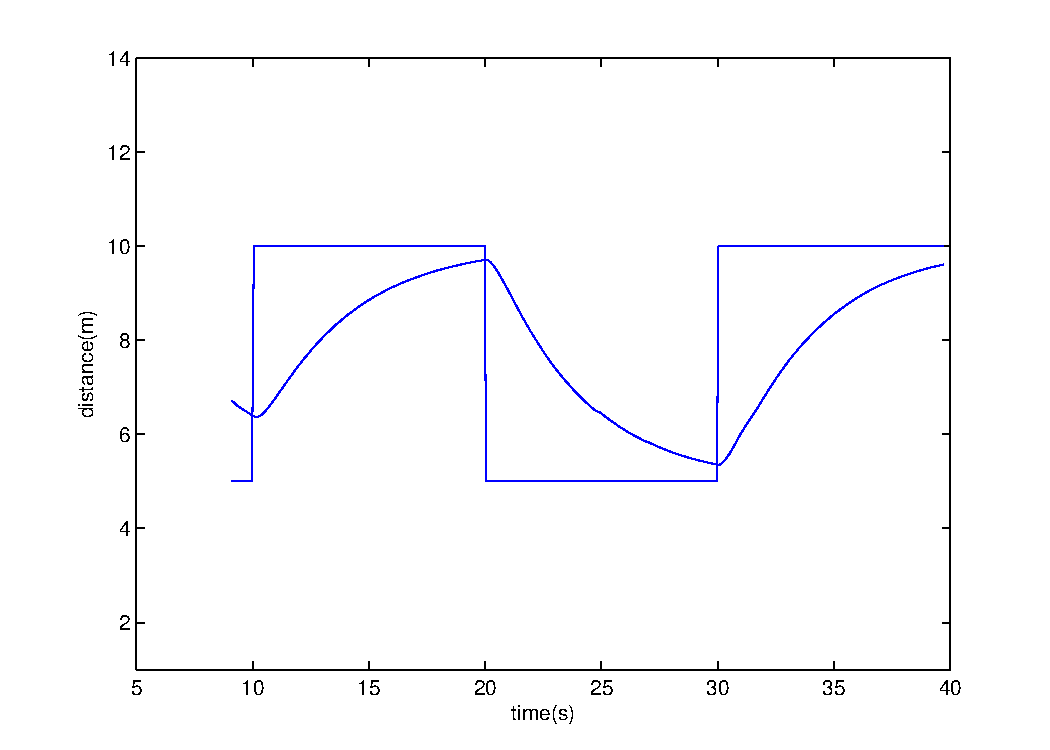
\includegraphics[width=\textwidth]{fig/gain1d1.pdf}
%                \caption{g 1, d 1}
%                \label{fig:gull}
%        \end{subfigure}%
%        ~ %add desired spacing between images, e. g. ~, \quad, \qquad, \hfill etc.
%          %(or a blank line to force the subfigure onto a new line)
%        \begin{subfigure}[b]{0.3\textwidth}
%                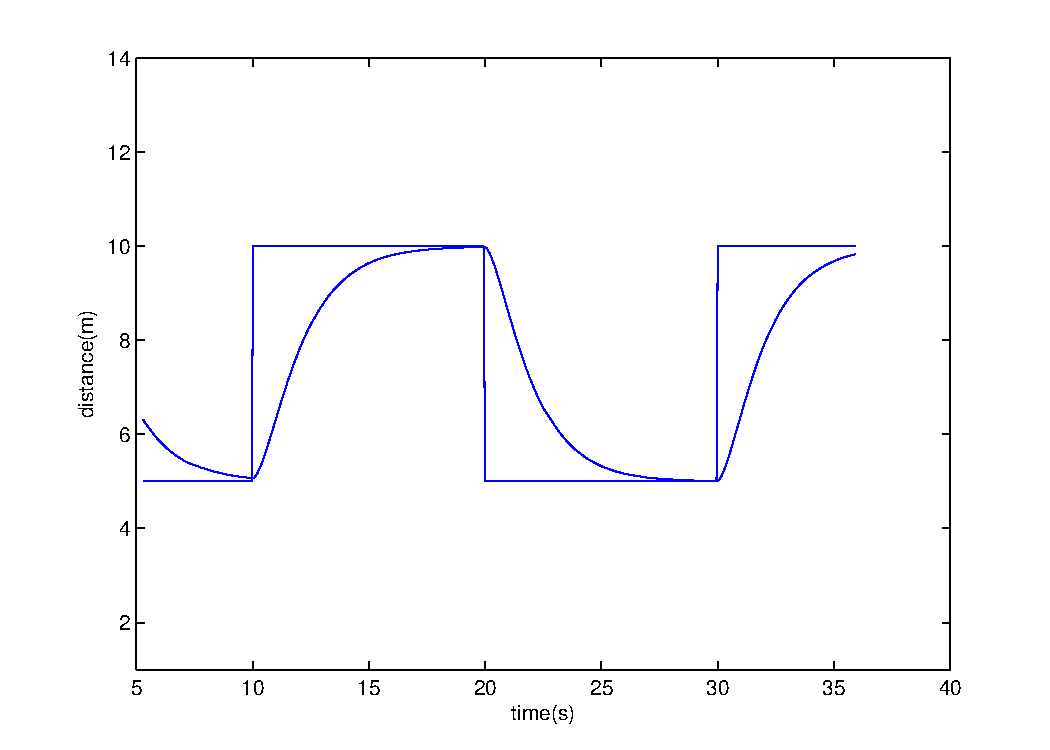
\includegraphics[width=\textwidth]{fig/gain2d1.pdf}
%                \caption{g 2, d 1}
%                \label{fig:tiger}
%        \end{subfigure}
%        ~ %add desired spacing between images, e. g. ~, \quad, \qquad, \hfill etc.
%          %(or a blank line to force the subfigure onto a new line)
%        \begin{subfigure}[b]{0.3\textwidth}
%                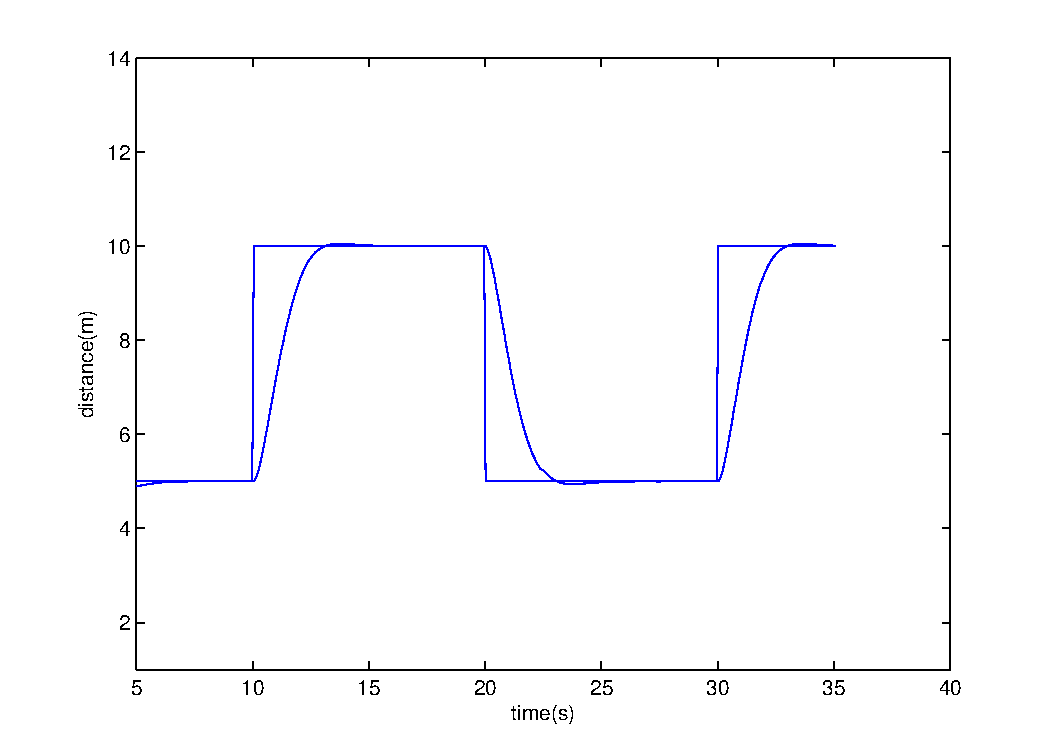
\includegraphics[width=\textwidth]{fig/gain4d1.pdf}
%                \caption{g 4, d 1}
%                \label{fig:mouse}
%        \end{subfigure}
%                \begin{subfigure}[b]{0.3\textwidth}
%                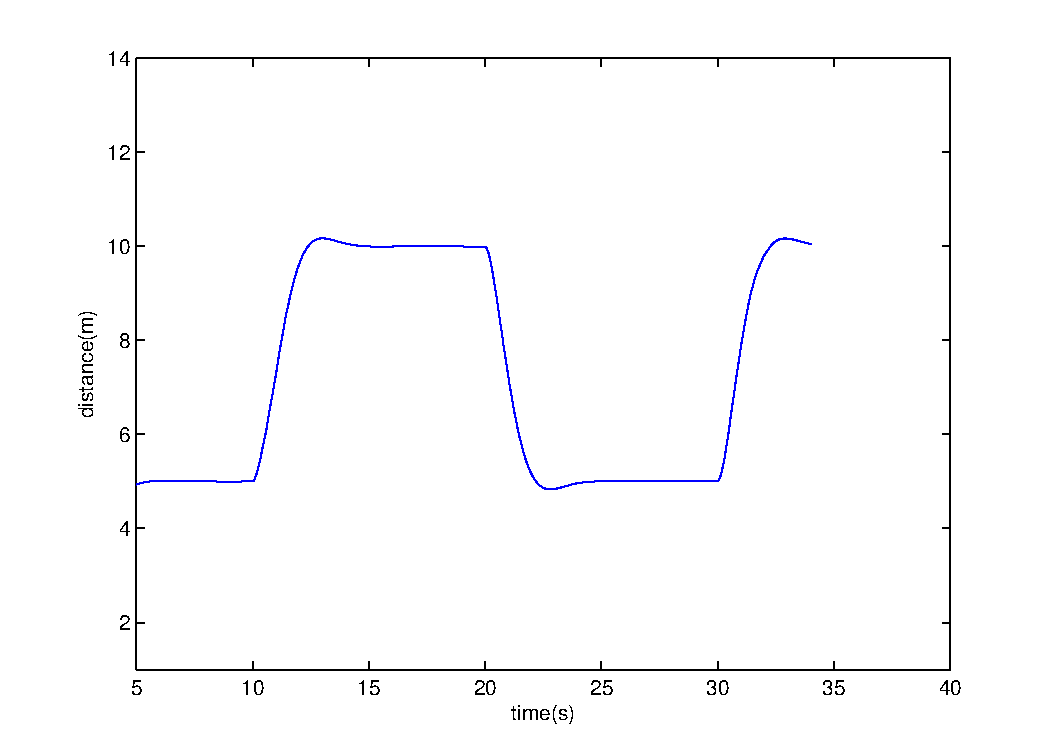
\includegraphics[width=\textwidth]{fig/gain5d1.pdf}
%                \caption{g 5, d 1}
%                \label{fig:gull}
%        \end{subfigure}%
%        ~ %add desired spacing between images, e. g. ~, \quad, \qquad, \hfill etc.
%          %(or a blank line to force the subfigure onto a new line)
%        \begin{subfigure}[b]{0.3\textwidth}
%                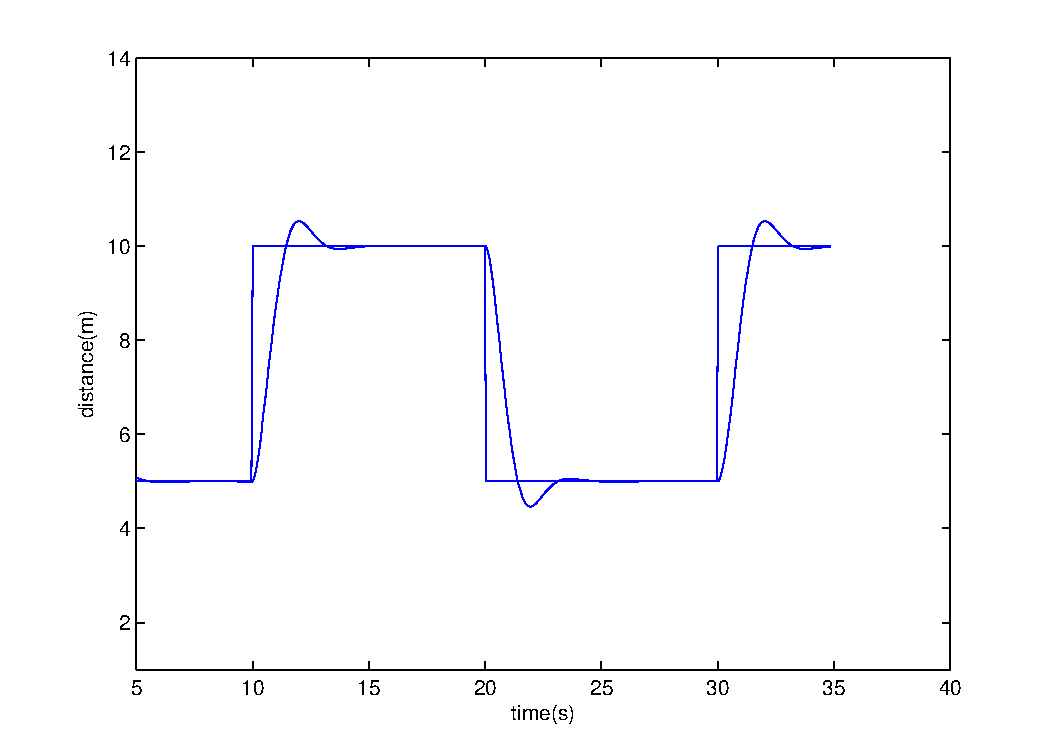
\includegraphics[width=\textwidth]{fig/gain8d1.pdf}
%                \caption{g 8, d 1}
%                \label{fig:tiger}
%        \end{subfigure}
%        ~ %add desired spacing between images, e. g. ~, \quad, \qquad, \hfill etc.
%          %(or a blank line to force the subfigure onto a new line)
%        \begin{subfigure}[b]{0.3\textwidth}
%                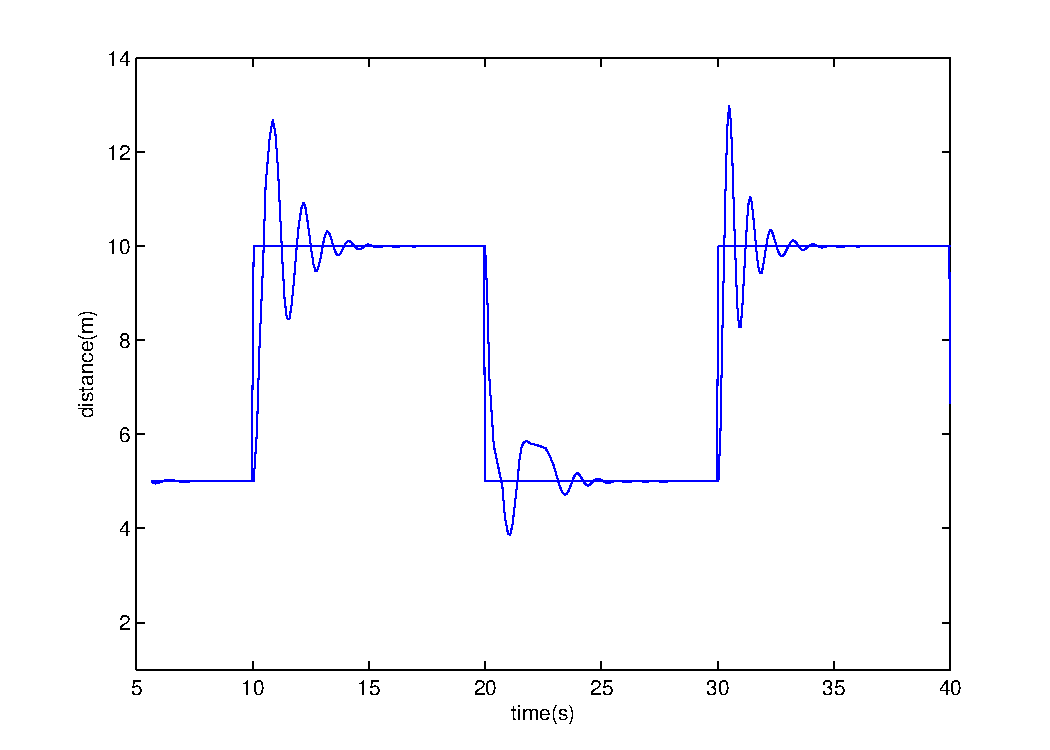
\includegraphics[width=\textwidth]{fig/gain100d1.pdf}
%                \caption{g 100, d 1}
%                \label{fig:mouse}
%        \end{subfigure}
%        \caption{Different Gain Values}\label{fig:gainvalues}
%\end{figure}
%\begin{figure}
%        \centering
%        \begin{subfigure}[b]{0.3\textwidth}
%                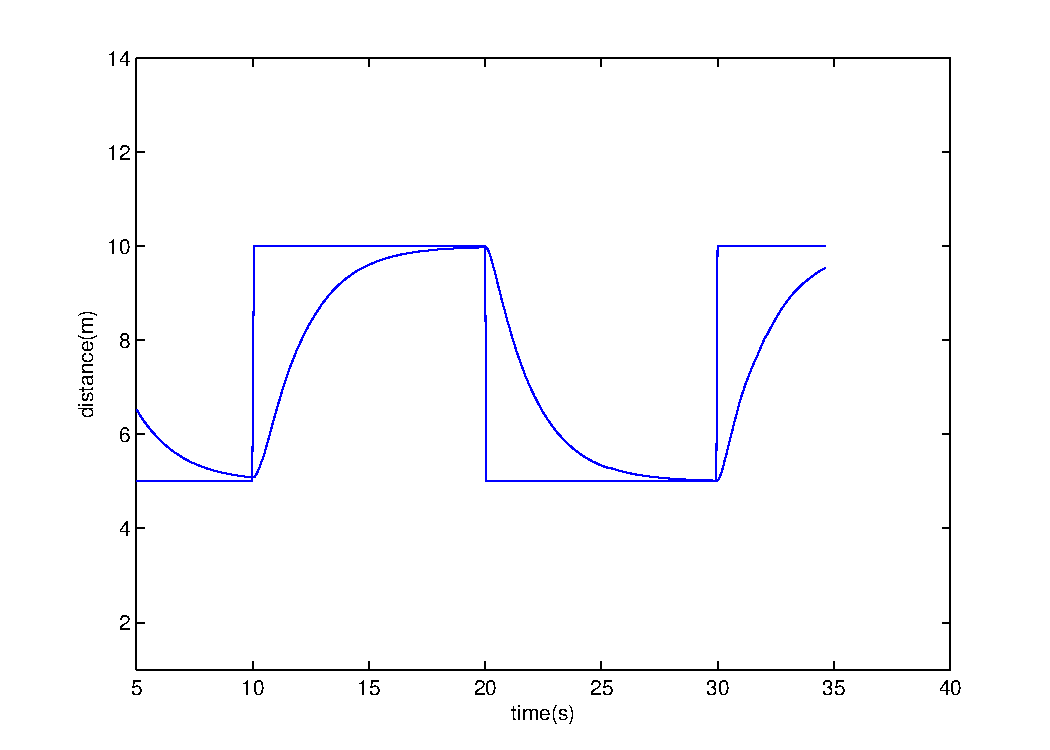
\includegraphics[width=\textwidth]{fig/gain4d2.pdf}
%                \caption{g 4, d 2}
%                \label{fig:gull}
%        \end{subfigure}%
%        ~ %add desired spacing between images, e. g. ~, \quad, \qquad, \hfill etc.
%          %(or a blank line to force the subfigure onto a new line)
%        \begin{subfigure}[b]{0.3\textwidth}
%                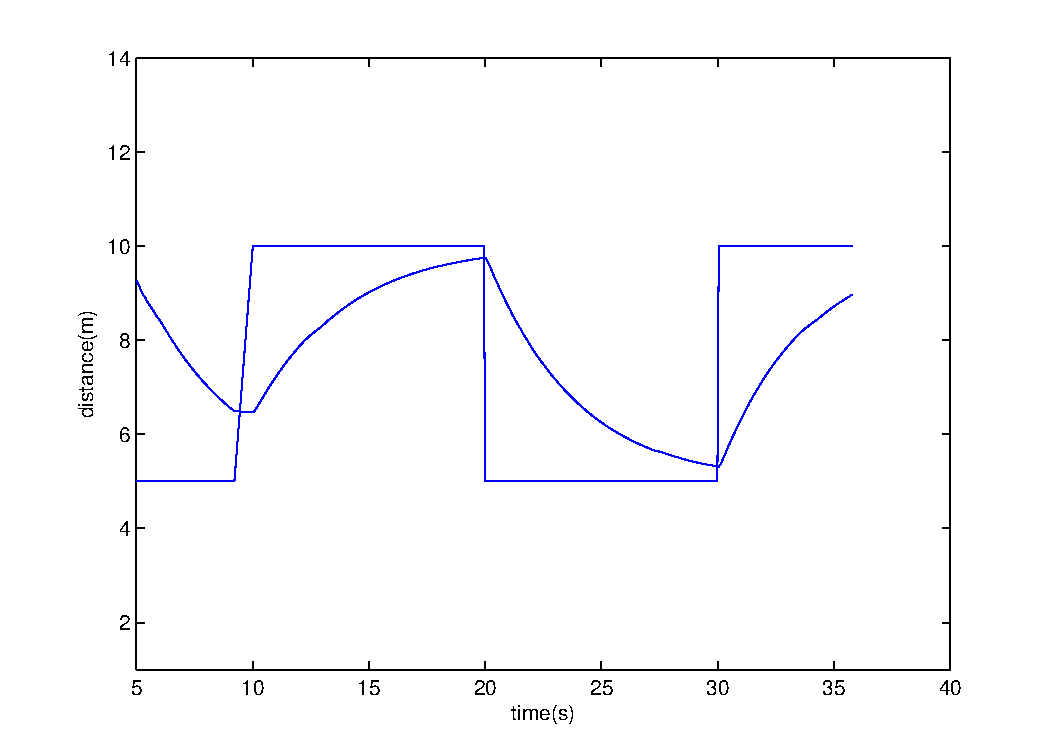
\includegraphics[width=\textwidth]{fig/gain4d4.pdf}
%                \caption{g 4, d 4}
%                \label{fig:tiger}
%        \end{subfigure}
%        ~ %add desired spacing between images, e. g. ~, \quad, \qquad, \hfill etc.
%          %(or a blank line to force the subfigure onto a new line)
%        \begin{subfigure}[b]{0.3\textwidth}
%                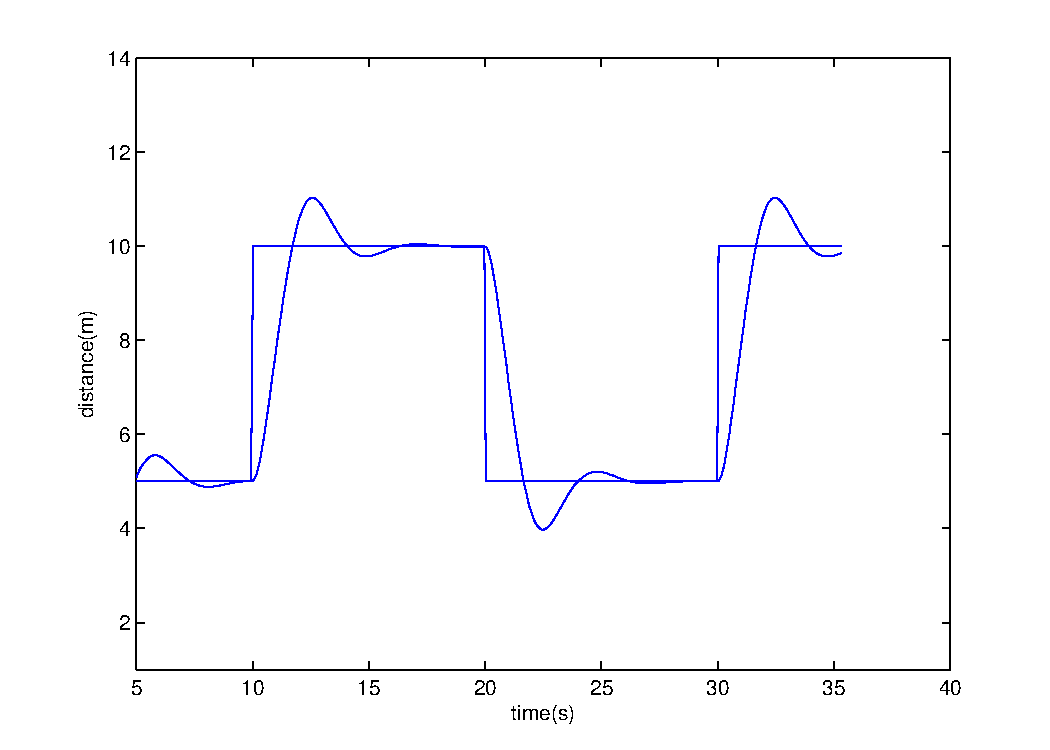
\includegraphics[width=\textwidth]{fig/gain4d05.pdf}
%                \caption{g 4, d 0.5}
%                \label{fig:mouse}
%        \end{subfigure}
%         \caption{Different Derivative Values}\label{fig:animals}
%\end{figure}


\subsection{Controlling the variance}

%cite the control law, explain experiment (number of robots, maximum speed, ).

For Controlling variance, as we discussed in section ???, we use a hysteresis variance control. For increasing variance we just need to wait and maybe it would be better to go to the area with less obstacles to speed up the process. And in order to decrease the variance, we go to corners to make the variance less.

%\begin{figure}[!htb]
%\captionsetup{justification=centering}
%\minipage{0.32\textwidth}
%  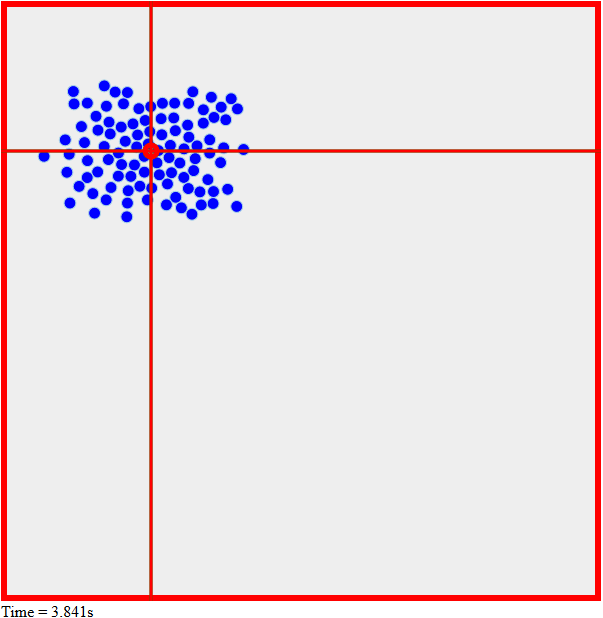
\includegraphics[width=\linewidth]{fig/2DControl3.png}
%  \caption{The goal position is 5 and 5}
%\endminipage\hfill
%\minipage{0.32\textwidth}
%  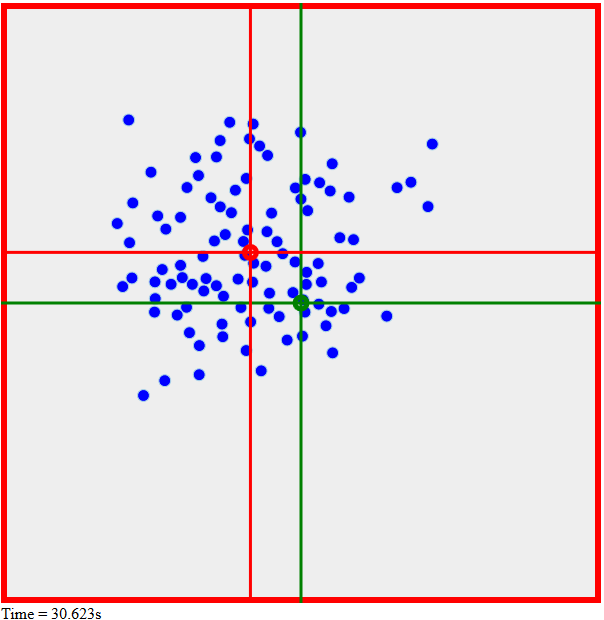
\includegraphics[width=\linewidth]{fig/2DControl2.png}
%  \caption{Going to the goal position}
%\endminipage\hfill
%\minipage{0.32\textwidth}%
%  %\includegraphics[width=\linewidth]{shiva444.eps}
%  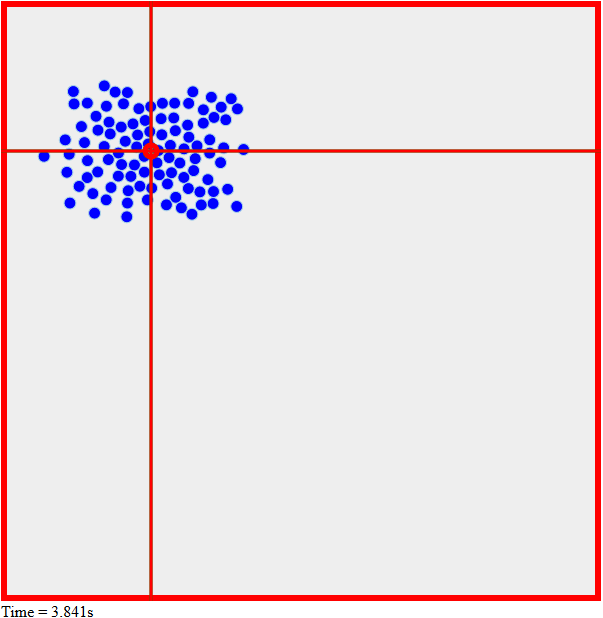
\includegraphics[width=\linewidth]{fig/2DControl3.png}
%  \caption{The goal position is 10 and 10}
%\endminipage
%\end{figure}
%\end{itemize}

contrast controllers -- as is typical with PID control laws, we can tune the response to meet desired specifications.

image showing varying Brownian noise

image showing control x variance and y-variance out of phase


\subsection{Hysteresis Control of mean and variance}

plot showing 1.5 cycles of mean position, and a variance goal.  We might need a longer time





